\chapter{PLANTEAMIENTO DEL PROBLEMA}
\section{Descripción de la Realidad Problemática}

El cobre, cuyo símbolo es Cu, se caracteriza por ser un elemento metálico maleable, dúctil y también un excelente conductor de calor y electricidad. Este metal se encuentra en nuestro planeta de forma natural en distintas formas. Se puede hallar en diferentes depósitos de minerales y en estado puro o dicho de otra forma «nativo» \parencite{cu_internationalcopper2018}. Esto último, es lo que lo vuelve un mineral atractivo, además de, una vez convertido en un producto terminado por las industrias, este puede ser empleado en el sector automovilístico, sector eléctrico, productos electrónicos, tecnologías de comunicación, construcciones, maquinaria industrial  y otros artículos de la vida cotidiana. %\medskip



\begin{figure}[h]
	\begin{center}
		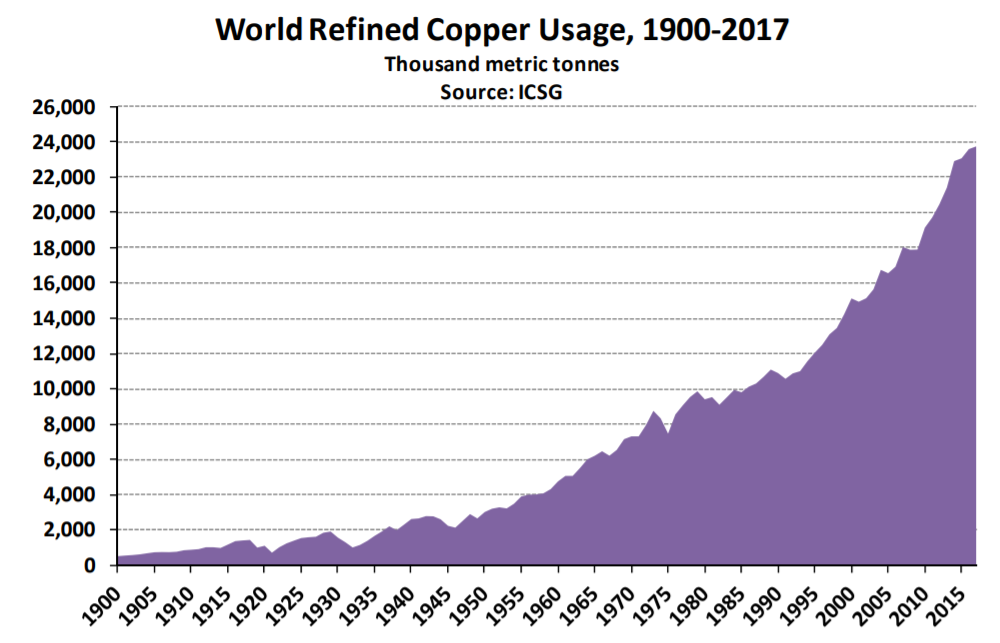
\includegraphics[width=0.8\textwidth]{1/figures/world_refined_copper_usage.png}
		\caption{Uso del cobre refinado mundial del año 1900 a 2017 (en miles de toneladas). Fuente: \cite{cu_internationalcopper2018}}
		\label{1:fig}
	\end{center}
\end{figure}

A lo largo de los años, como se observa en la Figura \ref{1:fig}, el uso del cobre refinado (cobre de alta pureza con una concentración de 99.9\%) en el mundo ha tenido un incremento bastante significativo y ello ha conllevado a un aumento en la comercialización de dicho metal. Como consecuencia, este ha contribuido en gran medida para las economías de diversas naciones ya sean países maduros o en vías de desarrollo. El minado, procesamiento, reciclaje y transformación de este metal a varios productos ha creado trabajos y generado riqueza. Estas actividades contribuyen en construir y mantener la infraestructura de un país, y además crea oportunidades de comercio e inversión \parencite{cu_internationalcopper2018}.



\begin{figure}[h]
	\begin{center}
		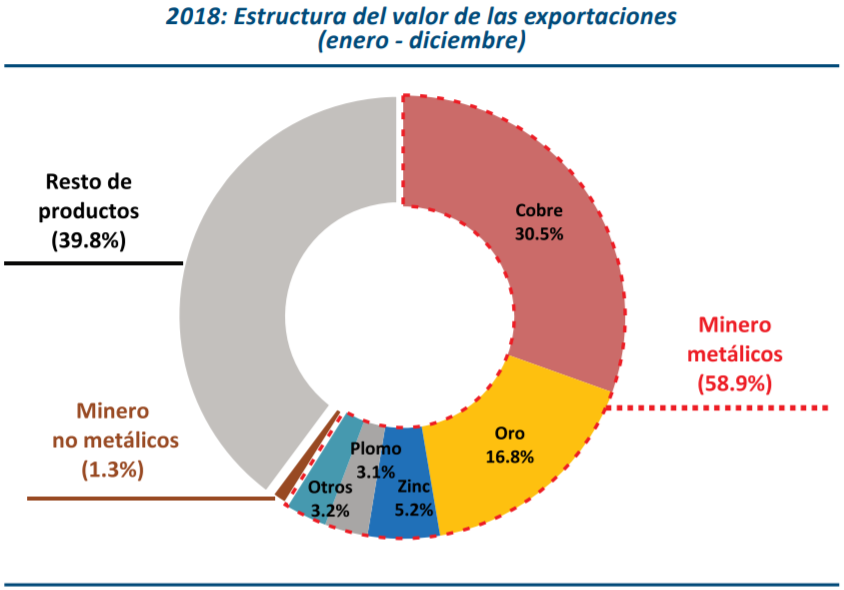
\includegraphics[width=0.8\textwidth]{1/figures/estructura_exportaciones_peru.png}
		\caption{Estructura del valor de las exportaciones peruanas en el año 2018. Fuente: \cite{cu_ministerioPeru_statsminas}}
		\label{1:fig2}
	\end{center}
\end{figure}




\begin{figure}[h]
	\begin{center}
		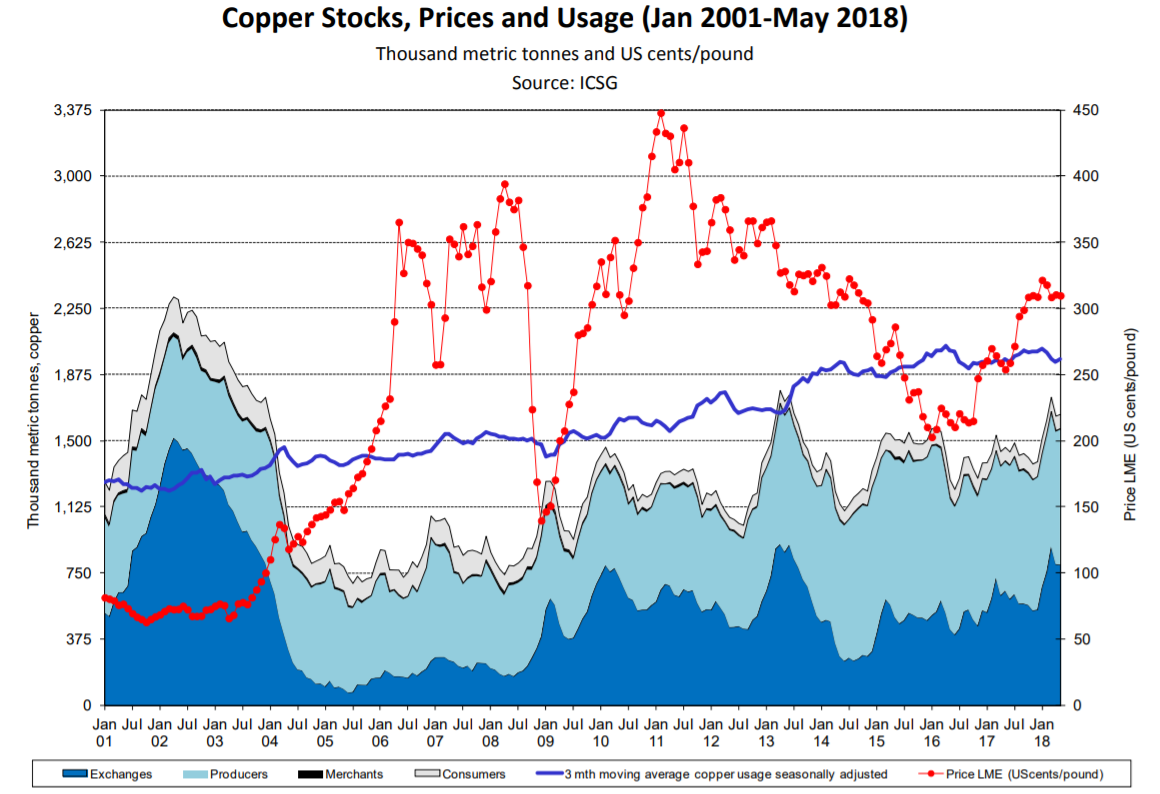
\includegraphics[width=0.8\textwidth]{1/figures/copper_stocks_prices_usage.png}
		\caption{Precio, stocks y uso del cobre (cantidad en miles de toneladas y precio en centavos por libra). Fuente: \cite{cu_internationalcopper2018}}	
		\label{1:fig3}
	\end{center}
\end{figure}

Estos modelos usados para predecir precios se basan mayormente en estimaciones de la oferta y demanda futura, así como los inventarios de bolsa. Otros consideran la memoria histórica de estas variables, la información de costos futuros de proyectos mineros, o variables financieras. Sin embargo, lo que estos modelos no hacen, es predecir el momento de la caída o alza del precio debido a eventos que no dependen de ninguna de las variables antes mencionadas sino a hechos inesperados globales \citep{cu_lagos2017proyectar}. 


\begin{figure}[h]
	\begin{center}
		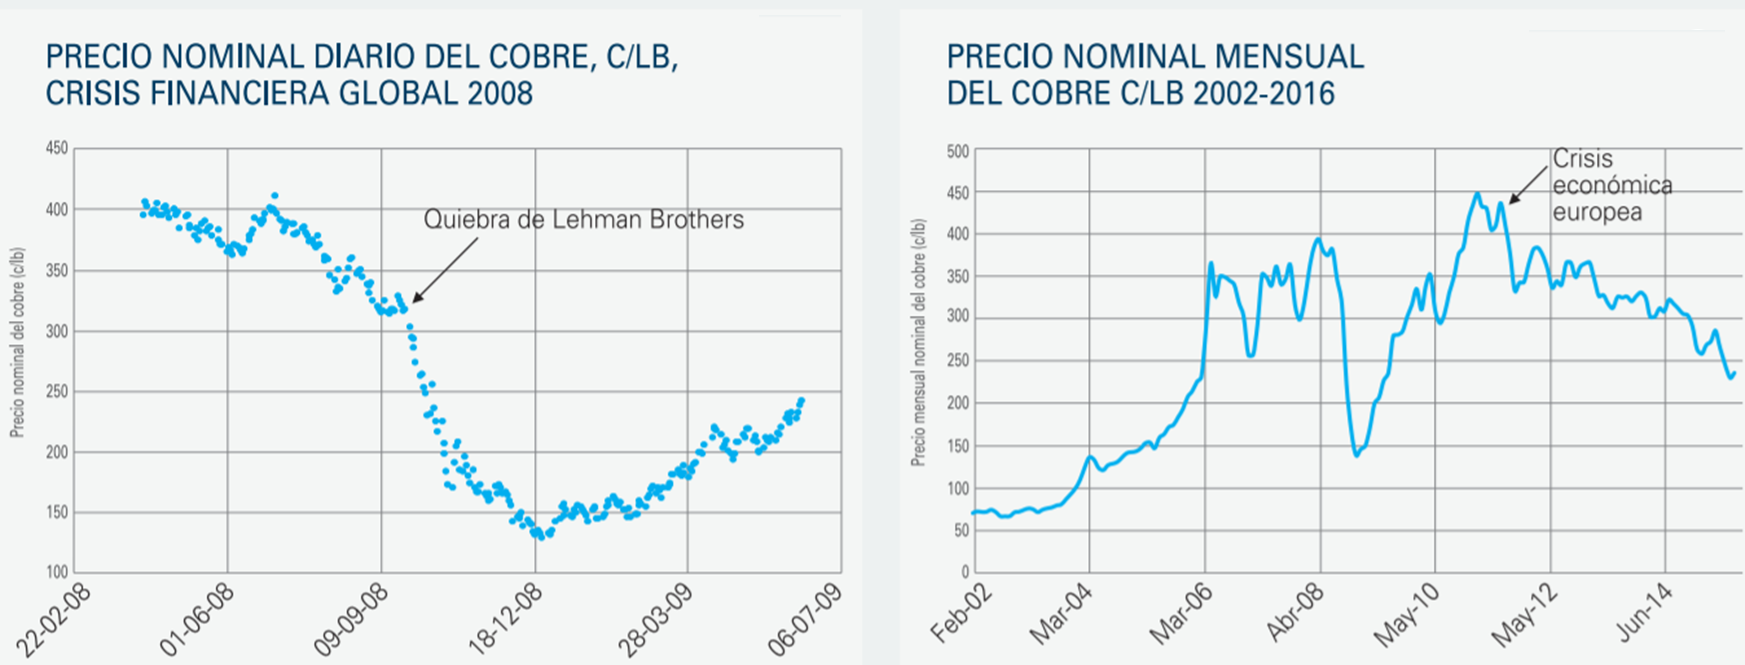
\includegraphics[width=0.8\textwidth]{1/figures/precio_caidas_gustavo_lagos.png}
		\caption{Precio, stocks y uso del cobre (cantidad en miles de toneladas y precio en centavos por libra). Fuente: \cite{cu_lagos2017proyectar}}
		\label{1:fig4}
	\end{center}
\end{figure} 




\section{Formulación del Problema}

Para lefecto \parencite{ot_marti2018manual}. 


Una vez elaborado el diagrama (véase Anexo 1), 

\subsection{Problema General}
\newcommand{\ProblemaGeneral}{
	Imprecisión del pronóstico del precio del cobre debido a la influencia de acontecimientos globales inesperados de diversos niveles de impacto. 
}
\ProblemaGeneral
\subsection{Problemas Espec\'{i}ficos}
\newcommand{\Pbone}{
X
}
\newcommand{\Pbtwo}{
Y
}
\newcommand{\Pbthree}{
Z
}
\newcommand{\Pbfour}{
W
}
\newcommand{\Pbfive}{
	ES
}

\begin{itemize}
	\item \Pbone
	\item \Pbtwo
	\item \Pbthree
	\item \Pbfour
	\item \Pbfive
\end{itemize}

\section{Objetivos de la Investigación}
Para la formulación de los objetivos de la presente investigación se elaboró un «árbol de objetivos» (véase Anexo 2) 
\subsection{Objetivo General}
\newcommand{\ObjetivoGeneral}{
Realizar xxx
}
\ObjetivoGeneral
\subsection{Objetivos Espec\'{i}ficos}
\newcommand{\Objone}{
xxx
}
\newcommand{\Objtwo}{
ggfg
}
\newcommand{\Objthree}{
gfghghg
}
\newcommand{\Objfour}{
hhhg
}
\newcommand{\Objfive}{
ghhhg
}

\begin{itemize}
	\item {\Objone}
	\item {\Objtwo}
	\item {\Objthree}
	\item {\Objfour}
	\item {\Objfive}
\end{itemize}

\section{Justificación de la Investigación}

\subsection{Teórica}
Esta investigación se realiza 

\subsection{Práctica}
Al culminar la investigación 

\subsection{Metodológica}. 

\section{Delimitación del Estudio}

\subsection{Espacial}
Para la presente investigación 

\subsection{Temporal}
Los datos que serán necesari. 

\subsection{Conceptual}
Esta investigación se 

\section{Hipótesis}

\subsection{Hipótesis General}
\newcommand{\HipotesisGeneral}{
El uso de técnicas de.
}
\HipotesisGeneral
\subsection{Hipótesis Específicas}
\newcommand{\Hone}{
	x
}
\newcommand{\Htwo}{
	y
}
\newcommand{\Hthree}{
	z	
}
\newcommand{\Hfour}{
	cv
}
\newcommand{\Hfive}{
	xws
}
\begin{itemize}
	\item \Hone
	\item \Htwo
	\item \Hthree
	\item \Hfour
	\item \Hfive
\end{itemize}

\subsection{Matriz de Consistencia}
A continuación se presenta la matriz de consistencia elaborada para la presente investigación (véase Anexo \ref{1:table}).

